\chapter{Poincare Map}
In the case of a toroidal apparatus, the intersection between particle trajectories and constant $\phi$ cross-section is indicative of the different regions of phase space.

[w7x / ncsx poincare section]

To compute it, the evolution of a particle along the magnetic field $\textbf{B}$ will be described using the non-unitary cylindrical basis given by $B =\{\partial_R, \partial_\phi, \partial_Z\}$ of $\mathcal{M} = \mathbb{R}^+\times[0,2\pi[\times\mathbb{R}$. By taking into account only the center of the gyro-motion, the particle follow the curve $\gamma : \mathbb{R}\rightarrow\mathcal{M}$, $t \mapsto \gamma(t) = (R(t),\,\phi(t),\,Z(t))$ such that the tangent vector at each point is given by $\dot{\gamma}(t)= \textbf{B} = B^i\partial_i \in T_{\gamma(t)}\mathcal{M}$. This defines a family of curves. By specifying the initial point $\gamma(0) = \textbf{x}_0$, we can write~:
\begin{align*}
    \gamma(t) = \int_0^t\dot{\gamma}(s)ds + \textbf{x}_0,
\end{align*}
with the component of the tangent vector being~:
\begin{align*}
    \dot{\gamma}^i(t)= (\frac{dR}{dt},\,\frac{d\phi}{dt},\,\frac{dZ}{dt}) = (B^R, B^\phi, B^Z).
\end{align*}
On the condition that the sign of $B^\phi(R, \phi, Z)$ remains either positive or negative on $\gamma$ the map~:
\begin{align*}
    t(\phi) = \int \frac{dt}{d\phi}d\phi = \int_0^\phi \frac{1}{B^\phi}d\phi
\end{align*}
is one-to-one and onto and therefore defines a handy change of variable for which the $\phi$ evolution is linear. Indeed $\gamma$ can be re-parameterized as $\phi \mapsto \gamma(\phi) = (R(\phi),\,\phi,\,Z(\phi))$ with~$\dot{\gamma}$~:
\begin{align*}
    \dot{\gamma}^i(\phi) = (\frac{dR}{d\phi},\,1,\,\frac{dZ}{d\phi}) = (\frac{dR}{dt}\frac{dt}{d\phi},\,1,\,\frac{dZ}{dt}\frac{dt}{d\phi}) = (B^R/B^\phi,\, 1,\,B^Z/B^\phi).
\end{align*}

\begin{figure}[h!]
    \centering
    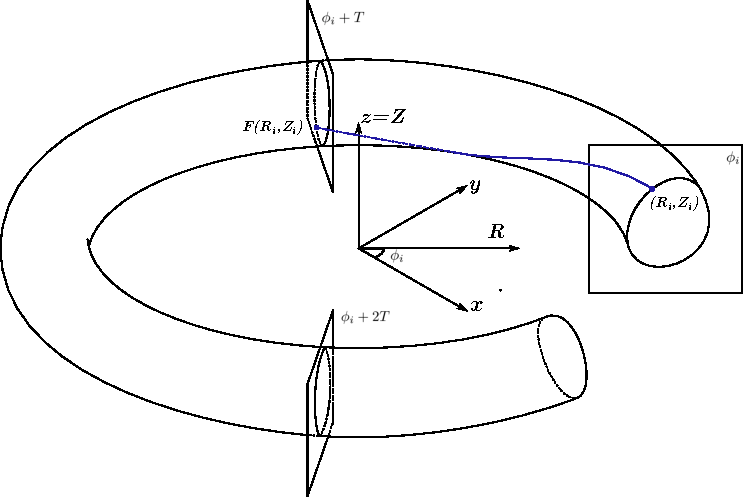
\includegraphics{images/theory/poincare-torus.pdf}
    \caption{Trajectory of a particle in a toroidal device (Tokamak/Stellarator) from a starting point $(\tilde{R}, \tilde{Z})$ in a $\phi = \phi_i$ section to a point in the $\phi = \phi_i + T$ plane with $T$ the azymuthal periodicity of the magnetic field.}
    \label{fig:poincare-map}
\end{figure}

The magnetic field has an azymuthal period $T = 2\pi/n_\text{fp}$ with $n_\text{fp}\in\mathbb{N}^\star$ the number of field period in a complete rotation. If the field is not periodic then $n_\text{fp} = 1$, on the contrary for an axisymmetric device without defaults $n_\text{fp} = +\infty$. The Poincare section is thus the same for $\phi_i$ and $\phi_i+kT$, $k\in\mathbb{Z}$. The Poincare map $F : \Omega \rightarrow \mathbb{R}_+\times\mathbb{R}$ is defined on $\Omega \subset \mathbb{R}_+\times\mathbb{R}$, the points for which the curve is indeed re-parametrizable between $\phi_i$ and $\phi_i + T$, by~:
\begin{align*}
    (\tilde{R},\tilde{Z}) \mapsto F(\tilde{R},\tilde{Z}) = \int_{\phi_i}^{\phi_i+T}(
        \dot{\gamma}^R(s),\,
        \dot{\gamma}^Z(s)
    )\,ds + (\tilde{R},\tilde{Z})
\end{align*}
with $\textbf{x}_0^i = (\tilde{R},\,\phi_i,\,\tilde{Z})$. 
the trajectory becomes $r_i$ with $z_{i+1} = F(z_i)$.

Note here that due to $\nabla\cdot\textbf{B} = 0$ the flux through any surface $A$ is the same as the one through $F(A)$~:
\begin{align*}
    \iint\limits_{A}\textbf{B}\cdot\textbf{dS} = \iint\limits_{F(A)}\textbf{B}\cdot\textbf{dS} \Leftrightarrow \int\limits_{A}\beta = \int\limits_{F(A)}\beta = \int\limits_{A}F^\star\beta
\end{align*}
where $\beta = i_Bdx^i\wedge dx^j$ is the flux form and $F^\star\beta$ the pullback of $\beta$ through the $F$ map, meaning that the poincare map is an area-preserving map for the flux for \cite{meiss_thirty_2015}. It implies on the determinant of the Jacobian $\textbf{DF} = \textbf{M}$ that given the identities~:
\begin{align*}
    \beta &= \beta_{ij}dx^i\wedge dx^j = \beta_{ij}dx^i\otimes dx^j\\
    F^\star\beta &= M^{i'}_{\,\:i}M^{j'}_{\,\:j}\beta_{i'j'}dx^i\wedge dx^j = \frac{1}{2}\beta_{i'j'}\left(M^{i'}_{\,\:i}M^{j'}_{\,\:j}-M^{i'}_{\,\:j}M^{j'}_{\,\:i}\right)dx^i\otimes dx^j\\ &= \frac{1}{2}\beta_{i'j'}\delta^{i'j'}_{ij} \det(\textbf{M})dx^i\otimes dx^j = \beta_{ij}\det(\textbf{M})dx^i\otimes dx^j
\end{align*}
that $\text{det}(\textbf{DF}(\tilde{R},\tilde{Z}))i_B(F(\tilde{R},\tilde{Z})) = i_B(\tilde{R},\tilde{Z})$. which can be seen as eq 8 from invariant in the case of a div free field. 

\section{Fixed point of the Poincare map}
The fixed point of $F$, $x\in\Omega$ such that $F(x) = x$, are of tw

X/O points are hyperbolic and elliptic points.

can be seen by viewing the into the poincare map paradigm by fixed point of F. The magnetic axis is one of such point with 

the rotational transform $\iota$ is the one also $q=m/n$.

Here the O/X-point of a q island is then a fixed-point the $F^p$ with $p = m//\gcd{m,n}$, 

the $\gcd{m,n}$ informs of how many different islands there are,

indeed take a $m/n$ island chain then by applying $lcm(m, n_fp)$ the map then we are back at the same point and have done $2\pi$


%%% -- CHAPTER --- %%%
\chapter{Toybox}
An analytical magnetic geometry is introduced to provide a simpler and more flexible approach to field line tracing analysis than treating the geometry of a complex toroidal device, as well as to validate the numerical calculation of further algorithms. Due to the linearity of the curl operator, a sum of vector potentials $\textbf{A}_i$ corresponds one-to-one to the element of the resulting magnetic fields $\textbf{B}_i$. A tokamak-like equilibrium is therefore implemented as the basis of this so-called \textit{Toybox}, to which perturbations can be added by summing their respective magnetic potential.

More specifically in axisymmetric equilibrium (i.e. perfect tokamaks), following e.g \cite[p.108]{wesson_tokamaks_2011}, the shape of the magnetic surfaces is well defined by the poloidal flux function $\psi$. Indeed, for cylindrical coordinates, all components/functions are constant along $\phi$, which yields~:
\begin{align*}
    \textbf{B} = B^i\partial_i = -\frac{1}{R}\frac{\partial\psi}{\partial Z}\partial_R +\frac{1}{R}\frac{\partial\psi}{\partial R}\partial_Z + \left(\frac{\partial A^R}{\partial Z} - \frac{\partial A^Z}{\partial R}\right)\partial_\phi.
\end{align*}
with $\psi = R^2 A^\phi$. The choice of Gauge can be exploited to assume $A^Z = 0$. For completeness, note that in the formulation of the Grad-Sharfranov equation, the $B^\phi$ term is related to a $F(\psi)$ flux function as $B^\phi = (\mu_0) F/R^2$.

A convenient geometry to study is nested toroidal flux surfaces centered on a magnetic axis of RZ-coordinates $(R_a, Z_a)$. Introducing toroidal coordinates $(\rho, \phi, \theta)$, where $\rho$ is the distance from the axis, the poloidal flux is thus $\psi(R, Z) \propto (R - R_a)^2 + (Z - Z_a)^2 = \rho^2$ and we will in fact take the equality due to the freedom of dimension in the implementation. For large aspect ratio tokamaks $R_a/\rho >> 1$ the safety factor profile can be approximated by~:
\begin{align*}
    q \approx \frac{\Delta\phi}{\Delta\theta} = \frac{\rho \tilde{B}^\phi}{R_a \tilde{B}^\theta} = \frac{2\pi}{\mu_0\tilde{I}^\phi R_a} \rho^2.
\end{align*}
Here the multipole expansion of $\tilde{B}^\theta$ is considered only up to first order. The $\tilde{B}^\phi$ component and the plasma current $\tilde{I}^\phi$ are imposed by the toroidal field coils and the central solenoid respectively. The q-profile is calculated more specifically by integrating along a flux tube in a phi cross section \cite[pp.111-112]{wesson_tokamaks_2011} as~:
\begin{align}\label{eq:q-profile-th}
    q(\rho) = \frac{1}{2\pi}\oint \frac{d\phi}{d\theta}d\theta = \frac{1}{2\pi}\oint \frac{B^\phi}{B^\theta}d\theta
\end{align}
Introducing heuristicaly the $\phi$ component of $\textbf{B}$ to be~:
\begin{align*}
    B^\phi = 2\sqrt{R^2-\rho^2}\,(\text{sf}+\text{shear}\rho^2)/R^2
\end{align*}
with corresponding $A^R$ given in [App1] and writing the transformation of the field to get the $\theta$ component~:
\begin{align*}
    B^\theta = \frac{\cos{\theta}}{\rho}B^Z - \frac{\sin{\theta}}{\rho}B^R = \frac{2}{R_a+\rho\cos{\theta}}
\end{align*}
finally inserting them into \eqref{eq:q-profile-th} gives~:
\begin{align*}
     q(\rho) = (\text{sf}+\text{shear}\rho^2)\frac{\sqrt{R^2-\rho^2}}{2\pi}\int\limits_{0}^{2\pi}\frac{1}{R_a + \rho\cos{\theta}}d\theta = \text{sf}+\text{shear}\rho^2
\end{align*}
the last integral is calculated analytically for $\rho < R$ the last two term cancel. \ref{fig:toytok-eq} shows the 

\begin{figure}[h!]
    \subfloat[First sub-figure]{%
        \label{fig:toytok-eq}
        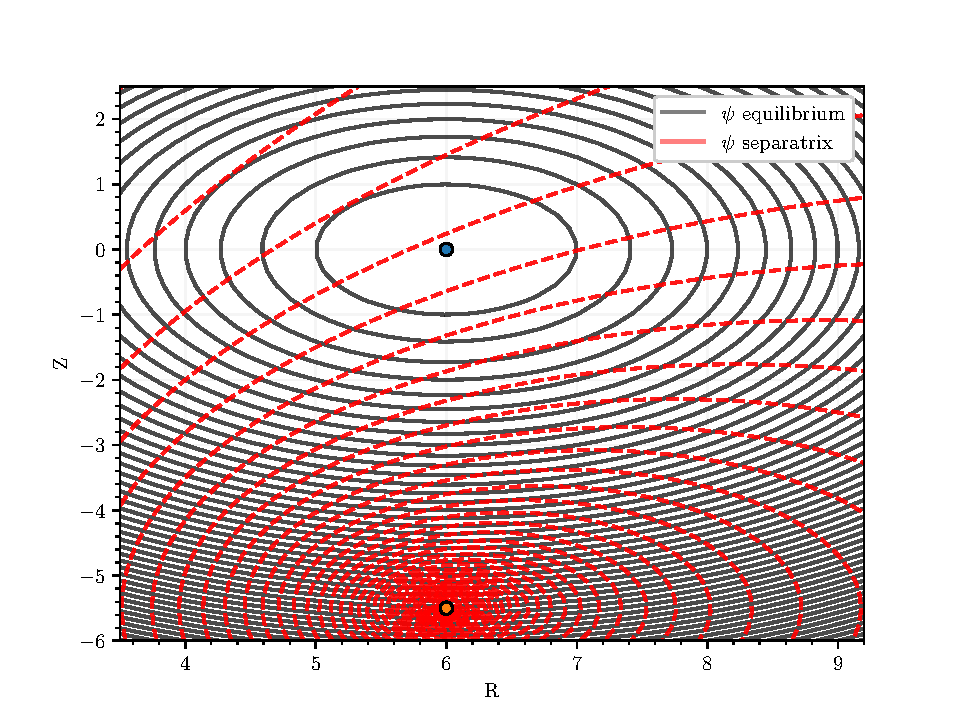
\includegraphics[width=0.33\textwidth]{images/plots/toytok/sepflux.pdf}
    }
    \subfloat[First sub-figure]{%
        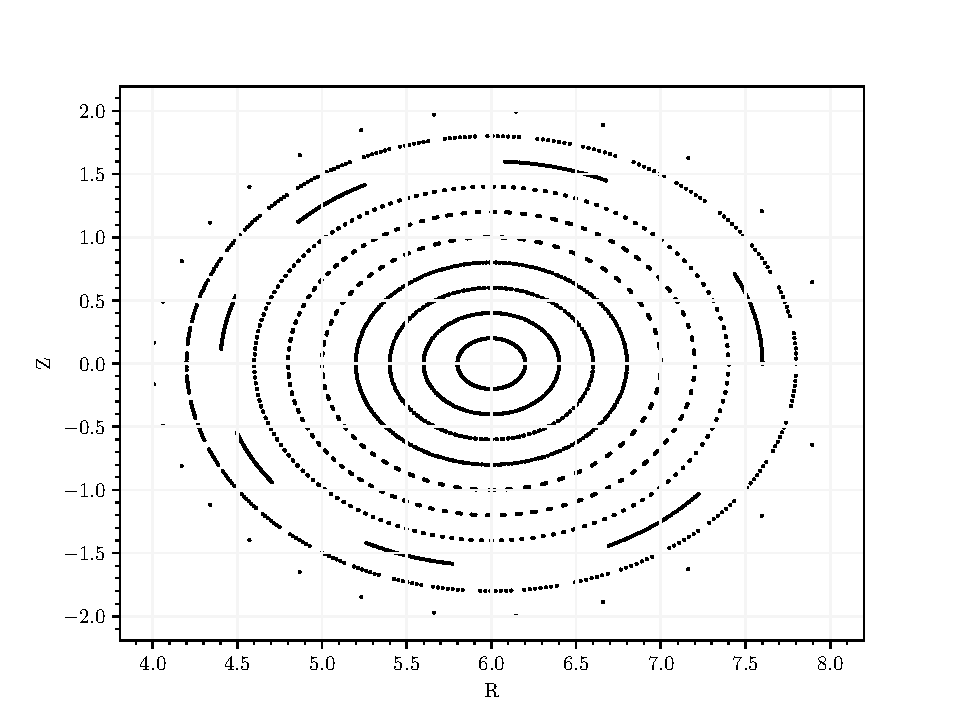
\includegraphics[width=0.33\textwidth]{images/plots/squared-profile/poincare.pdf}
    }
    \hfill
    \subfloat[First sub-figure]{%
        \label{fig:toytok-qprofile}
        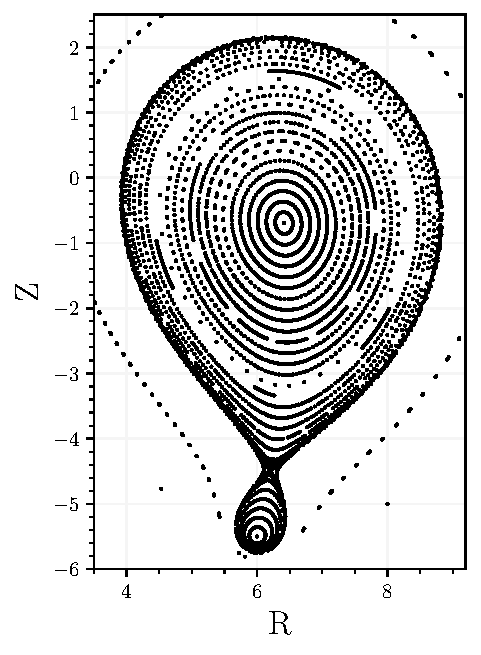
\includegraphics[width=0.33\textwidth]{images/plots/toytok/poincare.pdf}
    }
    \hfill
    \subfloat[First sub-figure]{%
        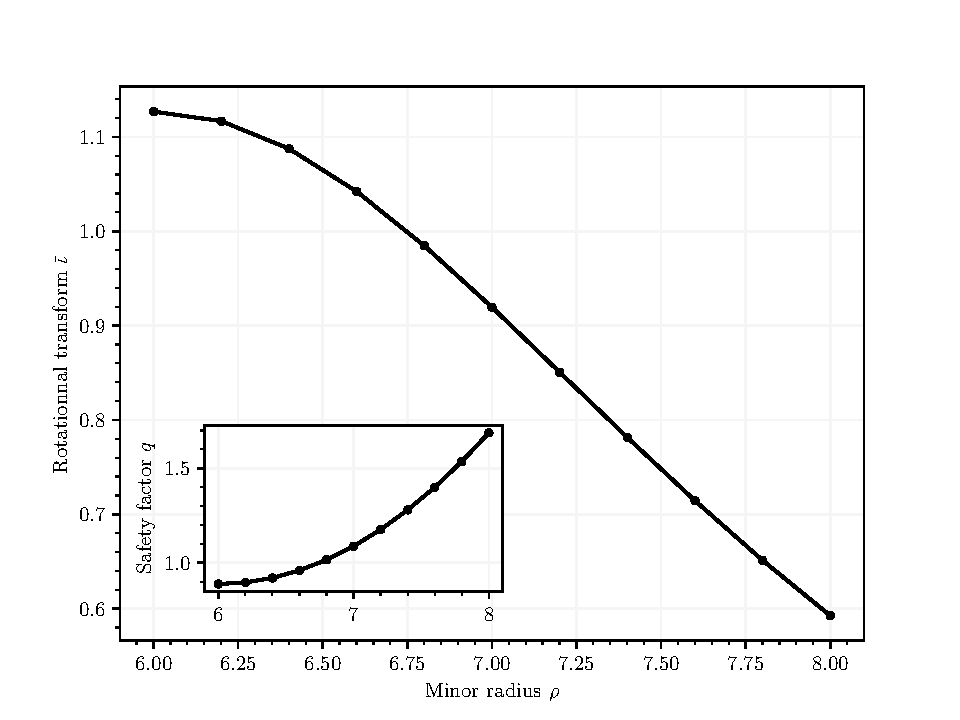
\includegraphics[width=0.45\textwidth]{images/plots/squared-profile/q-iota-squared.pdf}
    }
    \hfill
    \subfloat[First sub-figure]{%
        \includegraphics[width=0.45\textwidth]{example-image-c}
    }
    \caption{[toytok and toystell figure without perturbations]}
    \label{fig:toytok-toystell}
\end{figure}

A separatrix is essential to achieve a proper diverted tokamak structure. Combining the q-squared equilibrium with the field generated by a circular current loop at appropriate position and amplitude will produce the desired single null equilibrium. The vector potential of a loop at position $(0, a)$ is given in \cite{simpson_simple_2001} as~:
\begin{align*}
    A^\phi = \frac{\mu_0}{4\pi}\frac{4Ia}{\beta R}\left(\frac{(2-k^2)K(k^2)-2E(k^2)}{k^2}\right)
\end{align*}
with $\alpha^2 = a^2 + R^2 + Z^2 - 2aR$, $\beta^2 = a^2+R^2+Z^2+2aR$ and $k = 1 - \alpha^2/\beta^2$. we just need to shift the Z coordinates by $Z-a$.

give the iota/q-profiles of those, comparison with d3d or tcv for the reality of the toybox.

\section{Perturbations}
adding perturbation, not axisymmetric anymore. In the toroidal coordinates the $\phi$ and $\theta$ angles are both $\in [0, 2\pi)$ with $R_\text{max}(\theta)$ and thus one can develop any component into Fourier series as for the magnetic vector potential $\textbf{A}$.
\begin{align*}
    A^i(\rho,\phi,\theta) = \sum\limits_{n\in\mathbb{N}}\sum\limits_{m\in\mathbb{N}} A^i(\rho)\cos(n\phi + \varphi_n)\cos(m\theta + \varphi_m)
\end{align*}
One perturbation mode pair $(m,n)$ and remembering that the equilibrium is axisymmetric, thus one can choose the $\phi$ origin such that $\varphi_m = 0$, the perturbation becomes a choice of $\psi(\rho) = f(\rho)$.

Here the two choices~:

\begin{enumerate}
    \item $f(\rho, \mu, \sigma) = \frac{1}{\sqrt{2\pi\sigma^2}}\exp\left(\frac{-(\rho-\mu)^2}{2\sigma^2}\right)$ from the Normal distribution
    
    \item $f(\rho, d) = \frac{\sqrt{2}}{\sqrt{\pi}}\frac{\rho^2}{d^3}\exp\left(\frac{-\rho^2}{2d^2}\right)$ from the Maxwell-Boltzmann distribution
\end{enumerate}

In fact, the transformation to toroidal does not have to be the one of a circle. One can, for instance, find the flux coordinate for a tokamak equilibrium. Here only a generalization to an ellipsoid is implemented~:
\begin{align*}
    \rho &= \sqrt{\left(\frac{R-R_a}{A}\right)^2 + \left(\frac{Z-Z_a}{B}\right)^2}\\
    \phi &= \phi\\
    \theta &= \text{arctan2}(\frac{Z-Z_a}{B}, \frac{R-R_a}{A})\\
\end{align*}

talk about mode mixing : this is an choice in the way we apply the perturbation to mix mode.

[show some pertubations with the psi plot/mode mixing]

mode mixing is good because it create chaos fast, non definition of flux coordinate at the separatrix. The chaos appearing by ramping up the amplitude.

\chapter{Tangles and Turnstile}

[cite poincare]
from poincare also called them trellis [cite]
manifold, manifold ordering 

[plot of the manifold, toytok 6-1, toystell 3/2]

laking behind due to the q-profile

\section{Hetero/Homo-clinic points}
[floer homology from sonja]
what are they and algorithm to find them

higher order homoclinic points
[toytok 12-2, toystell 3/2]

\section{Turnstile}

the conservation, meiss

\subsection{Integration of the action}

The vector potential $\textbf{A} \in T\,\mathbb{R}^3$ is $\textbf{A} =  A^i\partial_i^\text{cyl}$.

$g = dR\otimes dR + R^2\,d\phi\otimes d\phi + dZ\otimes dZ$

The curvilinear integral of the scalar product $\textbf{A}\cdot\textbf{dl}$ along $\gamma$~:
\begin{align*}
    \int_0^\phi g(\textbf{A},\textbf{dl}) = \int_0^\phi g(\textbf{A}(\gamma(s)),\dot{\gamma}(s))ds\\ = \int_0^\phi (A^R\dot{\gamma}^R + R^2A^\phi\dot{\gamma}^\phi + A^Z\dot{\gamma}^Z) ds
\end{align*}
Thus for a $q=m/n=1/0$ fixed point of with $n_\text{fp} = 1$, it gives $2\pi R^2A^\phi = 2\pi R\tilde{A}^\phi$ with $\tilde{A}^\phi$ the $\phi$ component into the usual orthonormal cylindrical basis.

\begin{figure}[!ht]
    \subfloat[First sub-figure\label{subfig-1:dummy}]{%
      \includegraphics[width=0.45\textwidth]{example-image-a}
    }
    \hfill
    \subfloat[First sub-figure\label{subfig-2:dummy}]{%
      \includegraphics[width=0.45\textwidth]{example-image-b}
    }
    \caption{Dummy figure}
    \label{fig:turnstile-area-sketches}
\end{figure}

calculation and convergence

[toytok 6-1 with evolving and convergence, toystell same]
-